\section{Databasen}
\label{Technical_Database}

Vores endelige datamodel er illustreret af figur \ref{Fig:Technical_Database_datamodel} (side \pageref{Fig:Technical_Database_datamodel}). Vi har lavet en række ændringer til den datamodel, som er foreslået i kravspecifikationens kapitel \textit{D} \cite[s.14]{kravspec}. Denne datamodel er illustreret af figur \ref{Fig:Technical_Database_changes_KSdata} (side \pageref{Fig:Technical_Database_changes_KSdata}). Vi forklarer de ændringer, vi har lavet i afsnit \ref{Technical_Database_changes}.

\begin{figure}[h!]
  \centering
    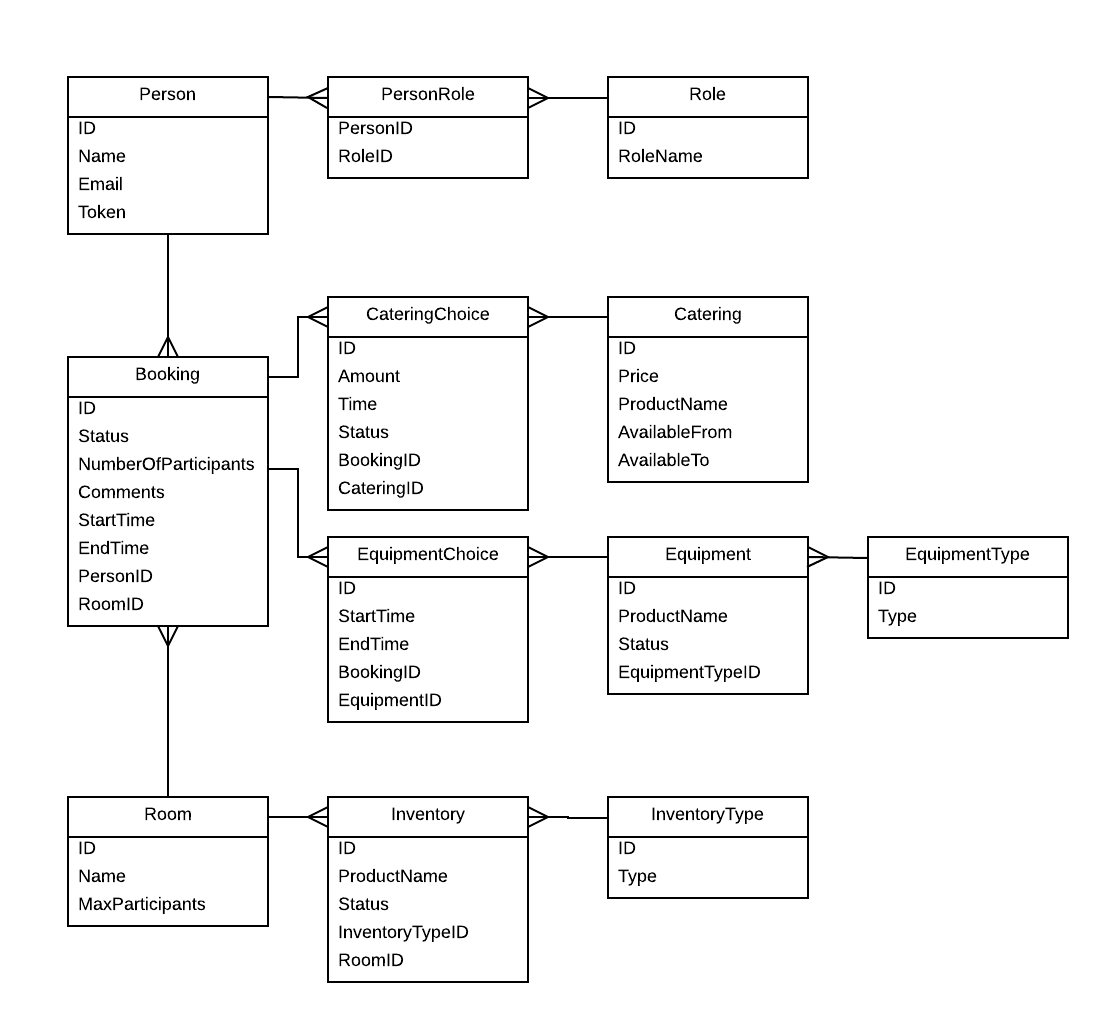
\includegraphics[width=\textwidth]{Chapters/Design/Technical/Images/OurDataModel}
  \caption{Datamodellen til vores løsning}
\label{Fig:Technical_Database_datamodel}
\end{figure}

\subsection{Ændringer til datamodellen}
\label{Technical_Database_changes}
\begin{figure}[h!]
  \centering
    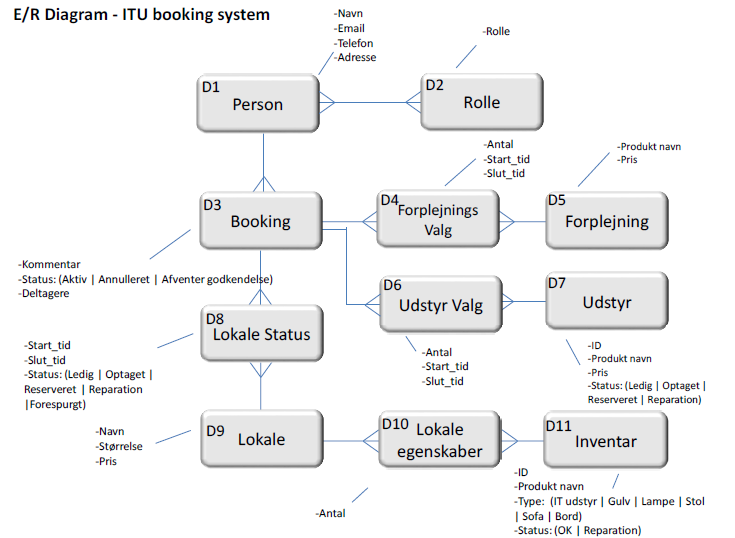
\includegraphics[width=\textwidth]{Chapters/Design/Technical/Images/KSdata}
  \caption{Kravspecifikationens datamodel}
\label{Fig:Technical_Database_changes_KSdata}
\end{figure}

\subsubsection{Personinformation}
\label{Technical_Database_changes_personinfo}
Det har primært været vores fokus at understøtte anvendelsen af IT-Universitetets Active Directory (AD) til at logge ind i systemet. Da ITUs AD ikke indeholder addresse eller telefonnummer, så inkluderer vi det ikke i vores datamodel. Dette kunne eventuelt indføres senere, hvis man ændrede i AD, brugte et andet system til godkende adgang eller lod brugeren redigere i sine data.

\subsubsection{Priser på lokaler/udstyr}
\label{Technical_Database_changes_prices}
Vi har valgt ikke at understøtte eksterne brugere i første release. Dette betyder, at det ikke er nødvendigt at inkludere priser på lokaler og udstyr. De kunne eventuelt blive introduceret som separate entiteter i databaser, således at priser kan justeres efter hvilken rolle, brugeren har i systemet.

\subsubsection{Lokale status}
\label{Technical_Database_changes_roomStatus}
Vi besluttede os for, at en booking kun kan bestå af et enkelt tidsrum og et enkelt lokale. Dette var hovedsageligt for at gøre det nemmere at implementere. Det gør det dog også nemmere at design brugergrænsefladen, da man ikke behøver lave et nyt skærmbillede i forbindelse med ændring af lokaler/tid til en booking.

\subsubsection{Forplejning}
\label{Technical_Database_changes_catering}
Vi lavede to ændringer i forbindelse med forplejning. Vi valgte at indføre et tidsrum, hvor et type forplejning var til rådighed. Dette gjorde vi, da vi gerne vil give køkkenet mulighed for at bestemme, om det fx skal være muligt at bestille morgenmad sent på eftermiddagen.
\\Den anden ændring var, at vi fjernede slut tiden på et forplejningsvalg. Vi mener ikke, det er nødvendigt at specificere, hvornår man er færdig med forplejning.

\subsubsection{Inventar- og udstyrstyper}
\label{Technical_Database_changes_types}
I stedet for at enumerere de forskellige typer af inventar og udstyr har vi oprettet en to type entiteter. Dette gør det nemmere at udvide de typer, som systemet understøtter. Vi overvejede at kombinere type entiteterne, men vi valgte det fra, da vi foretrak overskueligheden i separate entiteter.

\subsubsection{Lokale egenskaber}
\label{Technical_Database_changes_roomProperties}
Vi har fjernet lokale egenskaber i vores datamodel. Vi gør dette, fordi vi ser elementer i \textit{Inventar} entiteten som individuelle stykker inventar. Derfor kan der ikke være to af det samme stykke inventar, og dermed er \textit{Lokale} til \textit{Inventar} en "en til mange" relation.
\\Det samme gælder i udstyrsvalg - her har vi dog bare fjernet \textit{antal} attributten.

\subsubsection{Udstyr}
\label{Technical_Database_changes_ie}
Inventar og udstyr ligner hinanden meget efter, at vi har fjernet pris fra udstyr. Vi overvejede at lægge dem sammen til en enkelt entitet med en attribut, der angav, om produktet var til udlejning eller inventar til lokaler. Denne overvejelse kom dog først efter, vi var begyndt at implementere systemet, så vi tog ikke denne ændring med i første udgave.

\subsubsection{Token}
\label{Technical_Database_changes_token}
Vi har tilføjet en \textit{Token} attribut til \textit{Person} entiteten. Vi anvender \textit{Token} i forbindelse med kald til vores service.